% Options for packages loaded elsewhere
\PassOptionsToPackage{unicode}{hyperref}
\PassOptionsToPackage{hyphens}{url}
%
\documentclass[
]{article}
\usepackage{lmodern}
\usepackage{amssymb,amsmath}
\usepackage{ifxetex,ifluatex}
\ifnum 0\ifxetex 1\fi\ifluatex 1\fi=0 % if pdftex
  \usepackage[T1]{fontenc}
  \usepackage[utf8]{inputenc}
  \usepackage{textcomp} % provide euro and other symbols
\else % if luatex or xetex
  \usepackage{unicode-math}
  \defaultfontfeatures{Scale=MatchLowercase}
  \defaultfontfeatures[\rmfamily]{Ligatures=TeX,Scale=1}
\fi
% Use upquote if available, for straight quotes in verbatim environments
\IfFileExists{upquote.sty}{\usepackage{upquote}}{}
\IfFileExists{microtype.sty}{% use microtype if available
  \usepackage[]{microtype}
  \UseMicrotypeSet[protrusion]{basicmath} % disable protrusion for tt fonts
}{}
\makeatletter
\@ifundefined{KOMAClassName}{% if non-KOMA class
  \IfFileExists{parskip.sty}{%
    \usepackage{parskip}
  }{% else
    \setlength{\parindent}{0pt}
    \setlength{\parskip}{6pt plus 2pt minus 1pt}}
}{% if KOMA class
  \KOMAoptions{parskip=half}}
\makeatother
\usepackage{xcolor}
\IfFileExists{xurl.sty}{\usepackage{xurl}}{} % add URL line breaks if available
\IfFileExists{bookmark.sty}{\usepackage{bookmark}}{\usepackage{hyperref}}
\hypersetup{
  pdftitle={Kobe Bryant Shot Selection},
  pdfauthor={Laura Rodríguez Navas},
  hidelinks,
  pdfcreator={LaTeX via pandoc}}
\urlstyle{same} % disable monospaced font for URLs
\usepackage[margin=1in]{geometry}
\usepackage{color}
\usepackage{fancyvrb}
\newcommand{\VerbBar}{|}
\newcommand{\VERB}{\Verb[commandchars=\\\{\}]}
\DefineVerbatimEnvironment{Highlighting}{Verbatim}{commandchars=\\\{\}}
% Add ',fontsize=\small' for more characters per line
\usepackage{framed}
\definecolor{shadecolor}{RGB}{248,248,248}
\newenvironment{Shaded}{\begin{snugshade}}{\end{snugshade}}
\newcommand{\AlertTok}[1]{\textcolor[rgb]{0.94,0.16,0.16}{#1}}
\newcommand{\AnnotationTok}[1]{\textcolor[rgb]{0.56,0.35,0.01}{\textbf{\textit{#1}}}}
\newcommand{\AttributeTok}[1]{\textcolor[rgb]{0.77,0.63,0.00}{#1}}
\newcommand{\BaseNTok}[1]{\textcolor[rgb]{0.00,0.00,0.81}{#1}}
\newcommand{\BuiltInTok}[1]{#1}
\newcommand{\CharTok}[1]{\textcolor[rgb]{0.31,0.60,0.02}{#1}}
\newcommand{\CommentTok}[1]{\textcolor[rgb]{0.56,0.35,0.01}{\textit{#1}}}
\newcommand{\CommentVarTok}[1]{\textcolor[rgb]{0.56,0.35,0.01}{\textbf{\textit{#1}}}}
\newcommand{\ConstantTok}[1]{\textcolor[rgb]{0.00,0.00,0.00}{#1}}
\newcommand{\ControlFlowTok}[1]{\textcolor[rgb]{0.13,0.29,0.53}{\textbf{#1}}}
\newcommand{\DataTypeTok}[1]{\textcolor[rgb]{0.13,0.29,0.53}{#1}}
\newcommand{\DecValTok}[1]{\textcolor[rgb]{0.00,0.00,0.81}{#1}}
\newcommand{\DocumentationTok}[1]{\textcolor[rgb]{0.56,0.35,0.01}{\textbf{\textit{#1}}}}
\newcommand{\ErrorTok}[1]{\textcolor[rgb]{0.64,0.00,0.00}{\textbf{#1}}}
\newcommand{\ExtensionTok}[1]{#1}
\newcommand{\FloatTok}[1]{\textcolor[rgb]{0.00,0.00,0.81}{#1}}
\newcommand{\FunctionTok}[1]{\textcolor[rgb]{0.00,0.00,0.00}{#1}}
\newcommand{\ImportTok}[1]{#1}
\newcommand{\InformationTok}[1]{\textcolor[rgb]{0.56,0.35,0.01}{\textbf{\textit{#1}}}}
\newcommand{\KeywordTok}[1]{\textcolor[rgb]{0.13,0.29,0.53}{\textbf{#1}}}
\newcommand{\NormalTok}[1]{#1}
\newcommand{\OperatorTok}[1]{\textcolor[rgb]{0.81,0.36,0.00}{\textbf{#1}}}
\newcommand{\OtherTok}[1]{\textcolor[rgb]{0.56,0.35,0.01}{#1}}
\newcommand{\PreprocessorTok}[1]{\textcolor[rgb]{0.56,0.35,0.01}{\textit{#1}}}
\newcommand{\RegionMarkerTok}[1]{#1}
\newcommand{\SpecialCharTok}[1]{\textcolor[rgb]{0.00,0.00,0.00}{#1}}
\newcommand{\SpecialStringTok}[1]{\textcolor[rgb]{0.31,0.60,0.02}{#1}}
\newcommand{\StringTok}[1]{\textcolor[rgb]{0.31,0.60,0.02}{#1}}
\newcommand{\VariableTok}[1]{\textcolor[rgb]{0.00,0.00,0.00}{#1}}
\newcommand{\VerbatimStringTok}[1]{\textcolor[rgb]{0.31,0.60,0.02}{#1}}
\newcommand{\WarningTok}[1]{\textcolor[rgb]{0.56,0.35,0.01}{\textbf{\textit{#1}}}}
\usepackage{graphicx,grffile}
\makeatletter
\def\maxwidth{\ifdim\Gin@nat@width>\linewidth\linewidth\else\Gin@nat@width\fi}
\def\maxheight{\ifdim\Gin@nat@height>\textheight\textheight\else\Gin@nat@height\fi}
\makeatother
% Scale images if necessary, so that they will not overflow the page
% margins by default, and it is still possible to overwrite the defaults
% using explicit options in \includegraphics[width, height, ...]{}
\setkeys{Gin}{width=\maxwidth,height=\maxheight,keepaspectratio}
% Set default figure placement to htbp
\makeatletter
\def\fps@figure{htbp}
\makeatother
\setlength{\emergencystretch}{3em} % prevent overfull lines
\providecommand{\tightlist}{%
  \setlength{\itemsep}{0pt}\setlength{\parskip}{0pt}}
\setcounter{secnumdepth}{-\maxdimen} % remove section numbering

\title{\textbf{Kobe Bryant Shot Selection}}
\usepackage{etoolbox}
\makeatletter
\providecommand{\subtitle}[1]{% add subtitle to \maketitle
  \apptocmd{\@title}{\par {\large #1 \par}}{}{}
}
\makeatother
\subtitle{Proyecto Kaggle}
\author{Laura Rodríguez Navas}
\date{}

\begin{document}
\maketitle

\hypertarget{introducciuxf3n}{%
\section{\texorpdfstring{\textbf{Introducción}}{Introducción}}\label{introducciuxf3n}}

Este trabajo lleva a cabo un proyecto completo de Ciencia de Datos donde
vamos a analizar, transformar, modelar y evaluar un conjunto de datos de
\emph{Kaggle}. Concretamente, para este trabajo se ha usado un conjunto
de datos que describe los aciertos y los fallos de lanzamientos a
canasta del jugador de baloncesto Kobe Bryant durante los 20 años de su
carrera en la NBA
(\url{https://www.kaggle.com/c/kobe-bryant-shot-selection/data/}).

El conjunto de datos contiene 30697 instancias y un gran número de
variables explicativas (11 discretas y 14 numéricas). Estas 25 variables
(incluyendo clase a predecir \emph{``shot\_made\_flag''}) se centran en
la descripción cualitativa y cuantitativa de multitud de aspectos de
cada uno de los lanzamientos de Kobe Bryant.

\begin{verbatim}
## 'data.frame':    30697 obs. of  25 variables:
##  $ action_type       : Factor w/ 57 levels "Alley Oop Dunk Shot",..: 27 27 27 27 6 ..
##  $ combined_shot_type: Factor w/ 6 levels "Bank Shot","Dunk",..: 4 4 4 4 2 4 5 4 4 ..
##  $ game_event_id     : int  10 12 35 43 155 244 251 254 265 294 ...
##  $ game_id           : int  20000012 20000012 20000012 20000012 20000012 20000012 2..
##  $ lat               : num  34 34 33.9 33.9 34 ...
##  $ loc_x             : int  167 -157 -101 138 0 -145 0 1 -65 -33 ...
##  $ loc_y             : int  72 0 135 175 0 -11 0 28 108 125 ...
##  $ lon               : num  -118 -118 -118 -118 -118 ...
##  $ minutes_remaining : int  10 10 7 6 6 9 8 8 6 3 ...
##  $ period            : int  1 1 1 1 2 3 3 3 3 3 ...
##  $ playoffs          : int  0 0 0 0 0 0 0 0 0 0 ...
##  $ season            : Factor w/ 20 levels "1996-97","1997-98",..: 5 5 5 5 5 5 5 5 ..
##  $ seconds_remaining : int  27 22 45 52 19 32 52 5 12 36 ...
##  $ shot_distance     : int  18 15 16 22 0 14 0 2 12 12 ...
##  $ shot_made_flag    : int  NA 0 1 0 1 0 1 NA 1 0 ...
##  $ shot_type         : Factor w/ 2 levels "2PT Field Goal",..: 1 1 1 1 1 1 1 1 1 1 ..
##  $ shot_zone_area    : Factor w/ 6 levels "Back Court(BC)",..: 6 4 3 5 2 4 2 2 4 2 ..
##  $ shot_zone_basic   : Factor w/ 7 levels "Above the Break 3",..: 5 5 5 5 6 5 6 6 3..
##  $ shot_zone_range   : Factor w/ 5 levels "16-24 ft.","24+ ft.",..: 1 3 1 1 5 3 5 5..
##  $ team_id           : int  1610612747 1610612747 1610612747 1610612747 1610612747 ..
##  $ team_name         : Factor w/ 1 level "Los Angeles Lakers": 1 1 1 1 1 1 1 1 1 1 ..
##  $ game_date         : Factor w/ 1559 levels "1996-11-03","1996-11-05",..: 311 311 ..
##  $ matchup           : Factor w/ 74 levels "LAL @ ATL","LAL @ BKN",..: 29 29 29 29 ..
##  $ opponent          : Factor w/ 33 levels "ATL","BKN","BOS",..: 26 26 26 26 26 26 ..
##  $ shot_id           : int  1 2 3 4 5 6 7 8 9 10 ...
\end{verbatim}

La tarea de este trabajo es predecir si los lanzamientos a canastas de
Kobe Bryant entraron o no en el aro, es decir, los lanzamientos
acertados (atributo \emph{``shot\_made\_flag''}). Del conjunto de datos
se han eliminado 5000 valores de este atributo (representados como
valores faltantes). Estos datos estarán en el conjunto de evaluación
(test) sobre el cual se realizará la predicción.

\newpage

Una vez descargados los datos, es necesario dividir el conjunto de datos
en un conjunto de datos de entrenamiento y un conjunto de datos de
evaluación (test). Para ello, primero analizamos la existencia de esos
valores faltantes nombrados anteriormente (atributo
\emph{``shot\_made\_flag''}), que como hemos comentado serán los valores
que tendremos que predecir y que estarán en el conjunto de datos de test
pero no en el conjunto de datos de entrenamiento.

A continuación, podemos observar este proceso.

\begin{Shaded}
\begin{Highlighting}[]
\NormalTok{train <-}\StringTok{ }\NormalTok{data[}\OperatorTok{!}\KeywordTok{is.na}\NormalTok{(data}\OperatorTok{$}\NormalTok{shot_made_flag), ]}
\KeywordTok{any}\NormalTok{(}\KeywordTok{is.na}\NormalTok{(train))}
\end{Highlighting}
\end{Shaded}

\begin{verbatim}
## [1] FALSE
\end{verbatim}

\begin{verbatim}
##  int [1:25697] 0 1 0 1 0 1 1 0 0 1 ...
\end{verbatim}

\begin{Shaded}
\begin{Highlighting}[]
\NormalTok{test <-}\StringTok{ }\NormalTok{data[}\KeywordTok{is.na}\NormalTok{(data}\OperatorTok{$}\NormalTok{shot_made_flag), ]}
\KeywordTok{any}\NormalTok{(}\KeywordTok{is.na}\NormalTok{(test))}
\end{Highlighting}
\end{Shaded}

\begin{verbatim}
## [1] TRUE
\end{verbatim}

\begin{verbatim}
##  int [1:5000] NA NA NA NA NA NA NA NA NA NA ...
\end{verbatim}

Una vez dividido el conjunto de los datos, es necesario realizar un
análisis del conjunto de datos, así como un proceso de exploración,
transformación y limpieza de estos datos con el objetivo de resaltar
información útil para la fase de modelado. Este análisis nos permitirá
controlar la presencia de valores fuera de rango, una idea inicial de la
forma que tienen los datos, etc. así como las relaciones entre los
distintos atributos. Aunque para sintetizar el análisis realizado solo
se comentará aquello que se ha considerado más interesante durante éste.

\hypertarget{exploraciuxf3n-de-datos}{%
\section{\texorpdfstring{\textbf{Exploración de
datos}}{Exploración de datos}}\label{exploraciuxf3n-de-datos}}

Empezamos analizando visualmente la variable de clase a predecir
(atributo \emph{``shot\_made\_flag''}), que es binaria y que se
distribuye de manera bastante equitativa. Vemos que el número de
canastas que no entraron en el aro es superior al número de canastas que
sí que entraron. Así que, intentaremos averiguar si esto puede estar
relacionado con la gran lesión que tuvo Kobe Bryant durante la temporada
2013-14.

\begin{center}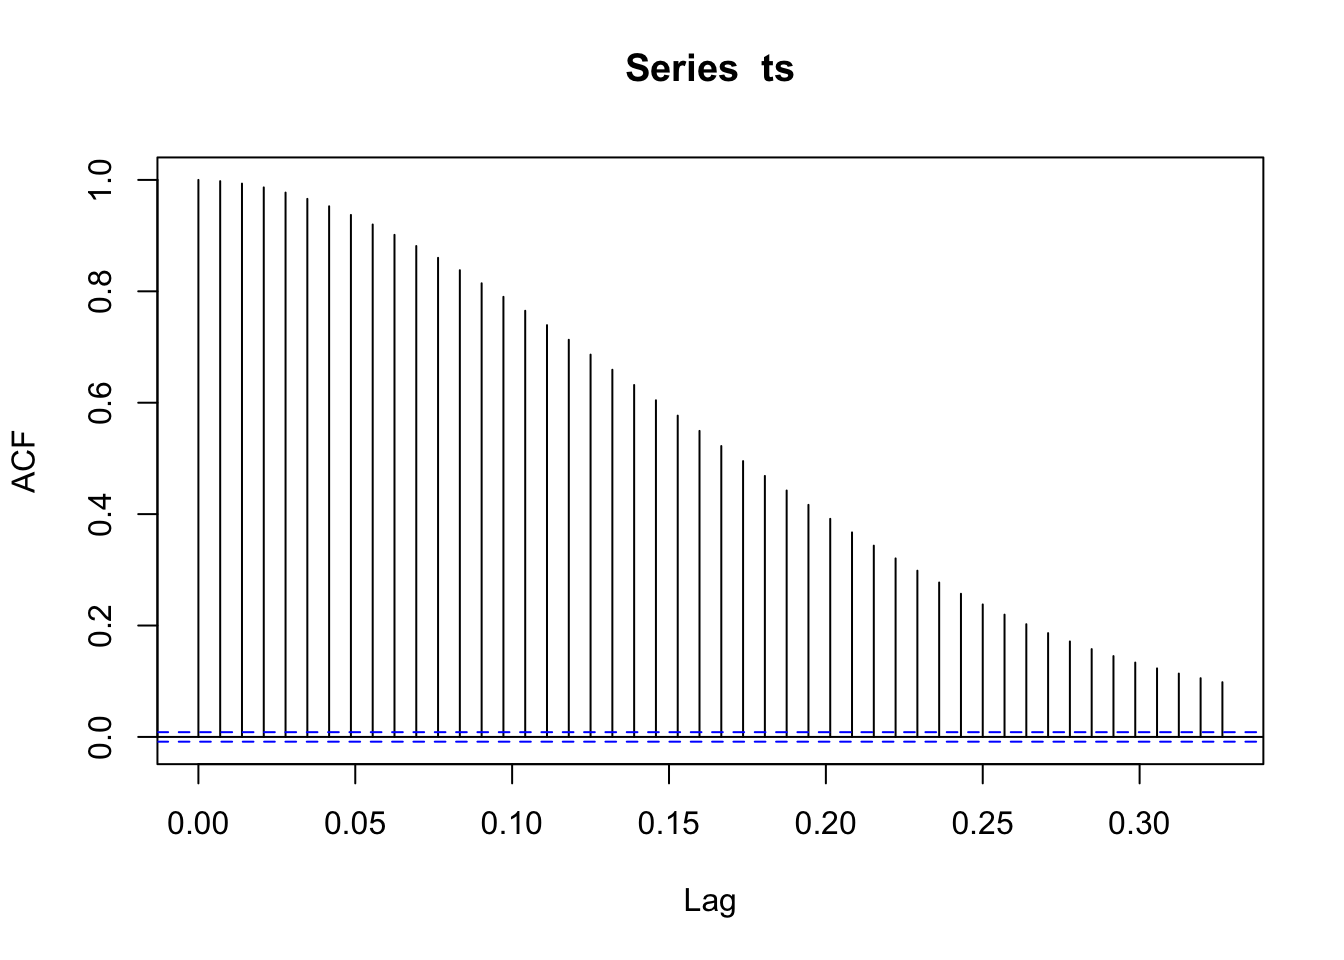
\includegraphics[width=0.6\linewidth]{document_files/figure-latex/unnamed-chunk-8-1} \end{center}

A continuación, analizamos visualmente la precisión de los lanzamientos
realizados por temporada (atributo \emph{``season''}), y vemos que a
partir de la temporada 2013-14 la precisión de los lanzamientos baja
drásticamente. ¿Así que, una gran cantidad de los lanzamientos que no
entraron en el aro están correlacionados a la gran lesión que tuvo en la
temporada 2013-14? Podría ser.

\begin{center}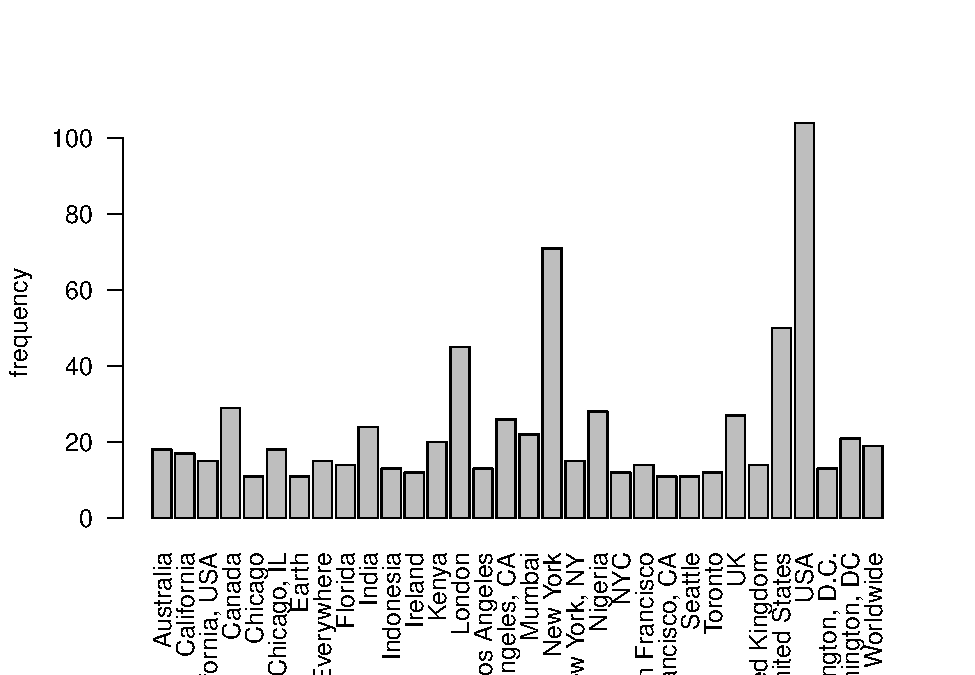
\includegraphics[width=0.7\linewidth]{document_files/figure-latex/unnamed-chunk-9-1} \end{center}

En el siguiente gráfico analizamos visualmente la precisión de los
lanzamientos respecto a la distancia de tiro (atributo
\emph{``shot\_distance''}), porqué en diferentes exploraciones de datos
que han realizado otros usuarios en \emph{Kaggle}, se ha podido observar
que el atributo \emph{``shot\_distance''} contiene valores fuera de
rango que podríamos eliminar en el apartado de limpieza de datos y que
nos sería muy beneficioso para reducir los fallos durante la predicción
en base a la distancia de los lanzamientos. Los valores fuera de rango
podrían encontrarse a partir de los lanzamientos realizados a más de 30
(ft.) ya que la precisión de estos baja drásticamente a partir de este
punto.

\begin{center}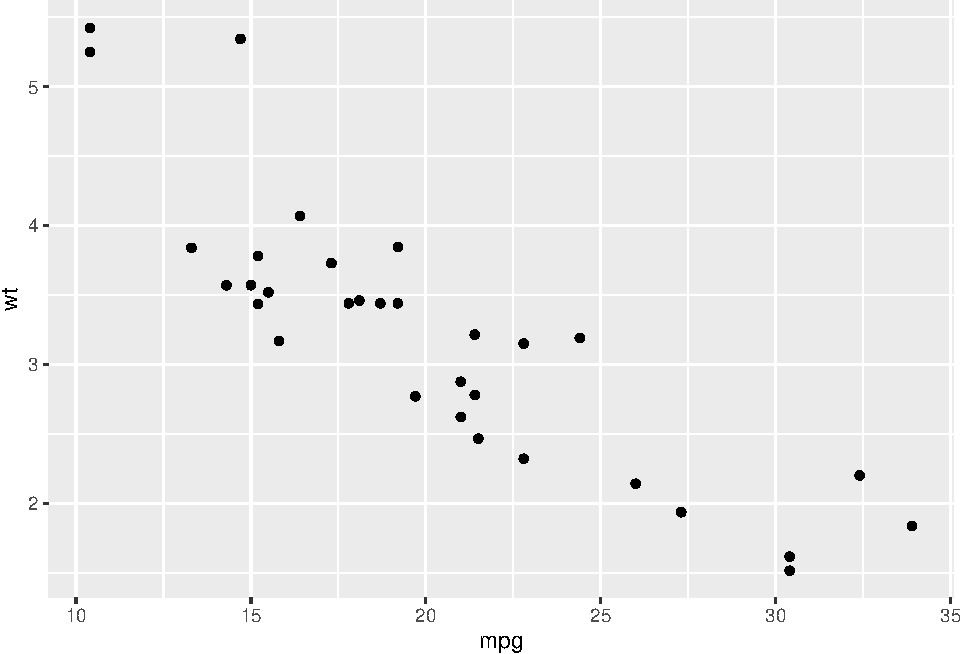
\includegraphics[width=0.7\linewidth]{document_files/figure-latex/unnamed-chunk-10-1} \end{center}

Y en siguiente grafico podemos observar la existencia de esos valores
fuera de rango que estábamos buscando, en el conjunto de datos de
entrenamiento. Y que valores exactamente se encuentran fuera de rango
son a partir de 40 (ft.). Así que, en el apartado de limpieza de datos
serán eliminados los valores del atributo \emph{shot\_distance}
superiores a 40 (ft.).

\begin{center}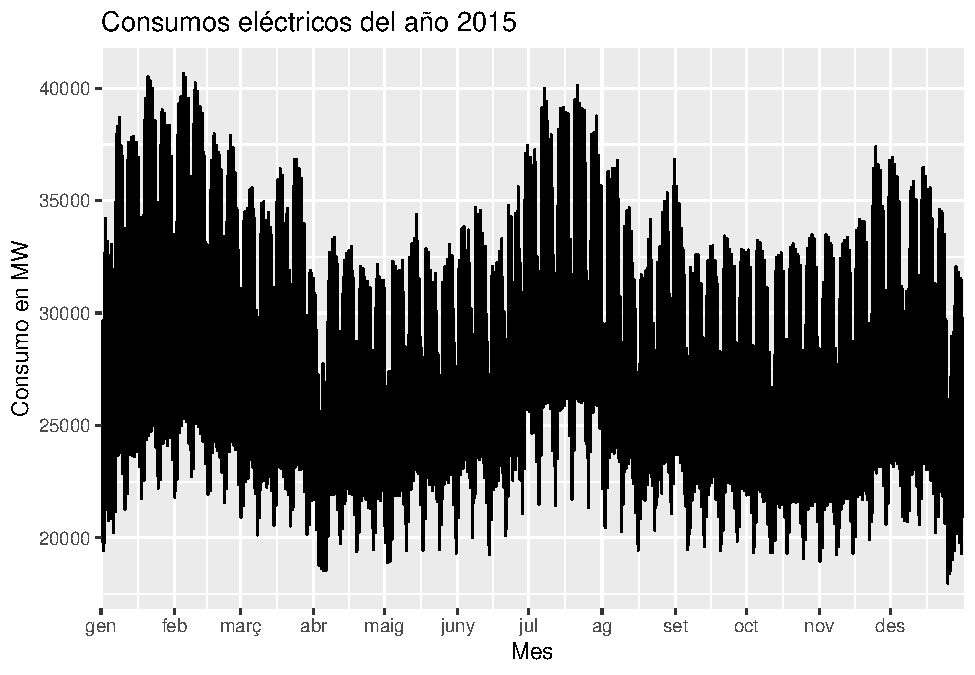
\includegraphics[width=0.7\linewidth]{document_files/figure-latex/unnamed-chunk-11-1} \end{center}

Anteriormente, hemos analizado visualmente la precisión de los
lanzamientos por temporada, los lanzamientos respecto a la distancia y
hemos encontrado valores fuera de rango en el conjunto de datos que
tendremos que eliminar si queremos realizar una buena predicción de la
variable clase \emph{``shot\_made\_flag''}.

Al trabajar con un conjunto de datos real, debemos tener en cuenta el
hecho de que algunos datos pueden faltar o estar dañados, por lo tanto,
es crucial realizar los procesos de transformación y limpieza del
conjunto de datos para obtener un buen ajuste del modelo y una mejor
capacidad predictiva.

\hypertarget{transformaciuxf3n-de-datos}{%
\section{\texorpdfstring{\textbf{Transformación de
datos}}{Transformación de datos}}\label{transformaciuxf3n-de-datos}}

La primera transformación que tenemos que realizar es la categorización
del atributo \emph{``shot\_made\_flag''}, porqué es la variable clase a
predecir e inicialmente es de tipo entero.

\begin{verbatim}
##  int [1:25697] 0 1 0 1 0 1 1 0 0 1 ...
\end{verbatim}

\begin{verbatim}
##  Factor w/ 2 levels "0","1": 1 2 1 2 1 2 2 1 1 2 ...
\end{verbatim}

Si nos fijamos en los atributos \emph{``minutes\_remaining''} y
\emph{``seconds\_remaining''} podríamos realizar la segunda
transformación sobre el conjunto de datos ya que la información que
contienen la podríamos combinar, los minutos del atributo
\emph{``minutes\_remaining''} los podríamos convertir a segundos y
sumar-los con los segundos del atributo \emph{``seconds\_remaining''}.
La nueva información combinada la guardaríamos en un nuevo atributo
\emph{``time\_remaining''}. El proceso se muestra a continuación.

\begin{Shaded}
\begin{Highlighting}[]
\NormalTok{train}\OperatorTok{$}\NormalTok{time_remaining <-}\StringTok{ }\NormalTok{train}\OperatorTok{$}\NormalTok{minutes_remaining }\OperatorTok{*}\StringTok{ }\DecValTok{60} \OperatorTok{+}\StringTok{ }\NormalTok{train}\OperatorTok{$}\NormalTok{seconds_remaining}
\NormalTok{test}\OperatorTok{$}\NormalTok{time_remaining <-}\StringTok{ }\NormalTok{test}\OperatorTok{$}\NormalTok{minutes_remaining }\OperatorTok{*}\StringTok{ }\DecValTok{60} \OperatorTok{+}\StringTok{ }\NormalTok{test}\OperatorTok{$}\NormalTok{seconds_remaining}
\end{Highlighting}
\end{Shaded}

Es importante hacer esta última transformación porqué después de
realizar la exploración del conjunto de datos, probar diferentes modelos
y explorar algunas soluciones encontradas en Kaggle se ha considerado
que la predicción se realizará sobre un conjunto de datos aún más
reducido que va a tener como atributos \emph{``time\_remaining''} y
\emph{``shot\_distance''}, además de la variable clase
\emph{``shot\_made\_flag''}. Para predecir sobre los lanzamientos
acertados según la distancia del lanzamiento durante períodos de tiempo.
Para ello también será necesaria la normalización de los atributos
(\emph{``time\_remaining''} y \emph{``shot\_distance''}) como podemos
ver a continuación.

\begin{Shaded}
\begin{Highlighting}[]
\NormalTok{normalize <-}\StringTok{ }\ControlFlowTok{function}\NormalTok{ (target) \{}
\NormalTok{  (target }\OperatorTok{-}\StringTok{ }\KeywordTok{min}\NormalTok{(target))}\OperatorTok{/}\NormalTok{(}\KeywordTok{max}\NormalTok{(target) }\OperatorTok{-}\StringTok{ }\KeywordTok{min}\NormalTok{(target))}
\NormalTok{\}}
\NormalTok{train}\OperatorTok{$}\NormalTok{shot_distance <-}\StringTok{ }\KeywordTok{normalize}\NormalTok{(train}\OperatorTok{$}\NormalTok{shot_distance)}
\NormalTok{test}\OperatorTok{$}\NormalTok{shot_distance <-}\StringTok{ }\KeywordTok{normalize}\NormalTok{(test}\OperatorTok{$}\NormalTok{shot_distance)}
\NormalTok{train}\OperatorTok{$}\NormalTok{time_remaining <-}\StringTok{ }\KeywordTok{normalize}\NormalTok{(train}\OperatorTok{$}\NormalTok{time_remaining)}
\NormalTok{test}\OperatorTok{$}\NormalTok{time_remaining <-}\StringTok{ }\KeywordTok{normalize}\NormalTok{(test}\OperatorTok{$}\NormalTok{time_remaining)}
\end{Highlighting}
\end{Shaded}

Todas las operaciones de transformación realizadas se han aplicado sobre
el conjunto de datos de entrenamiento y el conjunto de datos de test.

\hypertarget{limpieza-de-datos}{%
\section{\texorpdfstring{\textbf{Limpieza de
datos}}{Limpieza de datos}}\label{limpieza-de-datos}}

Durante la limpieza de datos vamos a eliminar los valores fuera de rango
que hemos encontrado durante la exploración del conjunto de datos y
eliminaremos los atributos que hemos creído independendientes al
modelado.

Comenzamos eliminando los valores fuera de rango, que como hemos visto
anteriormente una buena opción es descartar los lanzamientos por
distancia superiores a 40 (ft.). El proceso se muestra a continuación.

\begin{Shaded}
\begin{Highlighting}[]
\NormalTok{train}\OperatorTok{$}\NormalTok{shot_distance[train}\OperatorTok{$}\NormalTok{shot_distance }\OperatorTok{>}\StringTok{ }\DecValTok{40}\NormalTok{] <-}\StringTok{ }\DecValTok{40}
\NormalTok{test}\OperatorTok{$}\NormalTok{shot_distance[test}\OperatorTok{$}\NormalTok{shot_distance }\OperatorTok{>}\StringTok{ }\DecValTok{40}\NormalTok{] <-}\StringTok{ }\DecValTok{40}
\end{Highlighting}
\end{Shaded}

Y creemos que las siguientes columnas pueden descartarse.

\begin{itemize}
\tightlist
\item
  \textbf{game\_event\_id}. Independiente al modelado.
\item
  \textbf{game\_id}. Independiente al modelado.
\item
  \textbf{loc\_x}. Correlacionada con lat.
\item
  \textbf{loc\_y}. Correlacionada con lon.
\item
  \textbf{lat}. Correlacionada con loc\_x.
\item
  \textbf{lon}. Correlacionada con loc\_y.
\item
  \textbf{shot\_zone\_area}. Independiente al modelado.
\item
  \textbf{shot\_zone\_basic}. Independiente al modelado.
\item
  \textbf{shot\_zone\_range}. Independiente al modelado.
\item
  \textbf{team\_id}. Siempre es el mismo número.
\item
  \textbf{team\_name}. Siempre es el mismo valor: \emph{LA Lakers}.
\item
  \textbf{game\_date}. Independiente al modelado.
\item
  \textbf{matchup}. Los atributos \emph{oponent} y \emph{matchup}
  contienen básicamente la misma información. Nos quedamos solo con el
  atributo \emph{oponente}.
\item
  \textbf{minutes\_remaining}. Hemos combinado sus valores en una nueva
  columna (\emph{``time\_remaining''}) que contiene la misma
  información.
\item
  \textbf{seconds\_remaining}. Hemos combinado sus valores en una nueva
  columna (\emph{``time\_remaining''}) que contiene la misma
  información.
\end{itemize}

Después de la limpieza los conjuntos de datos de entrenamiento y de test
quedaron:

\begin{verbatim}
## 'data.frame':    25697 obs. of  11 variables:
##  $ action_type       : Factor w/ 57 levels "Alley Oop Dunk Shot",..: 27 27 27 6 27 ..
##  $ combined_shot_type: Factor w/ 6 levels "Bank Shot","Dunk",..: 4 4 4 2 4 5 4 4 4 ..
##  $ period            : int  1 1 1 2 3 3 3 3 3 1 ...
##  $ playoffs          : int  0 0 0 0 0 0 0 0 0 0 ...
##  $ season            : Factor w/ 20 levels "1996-97","1997-98",..: 5 5 5 5 5 5 5 5 ..
##  $ shot_distance     : num  0.19 0.203 0.278 0 0.177 ...
##  $ shot_made_flag    : Factor w/ 2 levels "0","1": 1 2 1 2 1 2 2 1 1 2 ...
##  $ shot_type         : Factor w/ 2 levels "2PT Field Goal",..: 1 1 1 1 1 1 1 1 2 1 ..
##  $ opponent          : Factor w/ 33 levels "ATL","BKN","BOS",..: 26 26 26 26 26 26 ..
##  $ shot_id           : int  2 3 4 5 6 7 9 10 11 12 ...
##  $ time_remaining    : num  0.871 0.651 0.577 0.531 0.801 ...
\end{verbatim}

\begin{verbatim}
## 'data.frame':    5000 obs. of  11 variables:
##  $ action_type       : Factor w/ 57 levels "Alley Oop Dunk Shot",..: 27 27 13 13 27..
##  $ combined_shot_type: Factor w/ 6 levels "Bank Shot","Dunk",..: 4 4 5 5 4 4 5 5 5 ..
##  $ period            : int  1 3 1 3 1 1 1 1 1 2 ...
##  $ playoffs          : int  0 0 0 0 0 0 0 0 0 0 ...
##  $ season            : Factor w/ 20 levels "1996-97","1997-98",..: 5 5 5 5 5 5 5 5 ..
##  $ shot_distance     : num  0.2951 0.0328 0 0 0.2787 ...
##  $ shot_made_flag    : int  NA NA NA NA NA NA NA NA NA NA ...
##  $ shot_type         : Factor w/ 2 levels "2PT Field Goal",..: 1 1 1 1 1 1 1 1 1 1 ..
##  $ opponent          : Factor w/ 33 levels "ATL","BKN","BOS",..: 26 26 31 31 32 32 ..
##  $ shot_id           : int  1 8 17 20 33 34 35 36 37 38 ...
##  $ time_remaining    : num  0.8831 0.6831 0.00141 0.90986 0.9662 ...
\end{verbatim}

Todas las operaciones de limpieza realizadas se han aplicado sobre el
conjunto de datos de entrenamiento y el conjunto de datos de test.

\hypertarget{modelado}{%
\section{\texorpdfstring{\textbf{Modelado}}{Modelado}}\label{modelado}}

Una vez se ha realizado la exploración, la transformación y la limpieza
de los datos, pasamos a la fase del modelado. Crearemos dos nuevos
conjuntos de datos sobre los conjuntos de datos de entrenamiento y el
conjunto de datos de test con los atributos (\emph{``time\_remaining''}
y \emph{``shot\_distance''}) y la variable de clase a predecir
(\emph{``shot\_made\_flag''}), que usaremos para obtener el modelo final
y hacer la predicción.

Los nuevos conjuntos de datos de entrenamiento y de test son:

\begin{verbatim}
## 'data.frame':    25697 obs. of  3 variables:
##  $ shot_distance : num  0.19 0.203 0.278 0 0.177 ...
##  $ time_remaining: num  0.871 0.651 0.577 0.531 0.801 ...
##  $ shot_made_flag: Factor w/ 2 levels "0","1": 1 2 1 2 1 2 2 1 1 2 ...
\end{verbatim}

\begin{verbatim}
##   shot_distance time_remaining shot_made_flag
## 1     0.1898734      0.8711485              0
## 2     0.2025316      0.6512605              1
## 3     0.2784810      0.5770308              0
## 4     0.0000000      0.5308123              1
## 5     0.1772152      0.8011204              0
\end{verbatim}

\begin{verbatim}
## 'data.frame':    5000 obs. of  3 variables:
##  $ shot_distance : num  0.2951 0.0328 0 0 0.2787 ...
##  $ time_remaining: num  0.8831 0.6831 0.00141 0.90986 0.9662 ...
##  $ shot_made_flag: int  NA NA NA NA NA NA NA NA NA NA ...
\end{verbatim}

\begin{verbatim}
##   shot_distance time_remaining shot_made_flag
## 1    0.29508197    0.883098592             NA
## 2    0.03278689    0.683098592             NA
## 3    0.00000000    0.001408451             NA
## 4    0.00000000    0.909859155             NA
## 5    0.27868852    0.966197183             NA
\end{verbatim}

Para decidir el modelo final probamos diferentes modelos que hemos ido
viendo durante la asignatura y que se recomendaban en Kaggle, sobre el
conjunto de datos de entrenamiento. Para quedarnos con el mejor modelo
usamos las matrices de confusión de cada modelo resultantes de las
predicciones sobre el conjunto de datos de entrenamiento para comparar
los valores de la métrica \emph{Accuracy} entre ellos. A continuación,
podemos observar una tabla con los valores de \emph{Accuracy} de los
modelos que se han probado.

\newpage

\begin{verbatim}
##                        Accuracy
## LDA                   0.5972292
## Naive Bayes           0.6083590
## Decision Tree         0.6099156
## Neural Network        0.6085924
## Nearest Neighbour     0.7203565
## SVM (linear kernel)   0.5879675
## Multilayer Perceptron 0.6076585
## Random Forest         0.8043351
## GLM                   0.9294118
\end{verbatim}

Como se observa en la tabla anterior, el mejor modelo es el modelo
lineal generalizado con un valor de \emph{Accuracy} de 0.9294118.
Concretamente, es el modelo binominal de regresión. Dentro de los
diferentes tipos de modelos lineales se escogió el modelo binominal
porqué la variable a predecir es binaria.

Este tipo de modelo ha funcionado tan bien porqué el problema que se nos
ha planteado tiene como objetivo aprender qué valores de las entradas
del conjunto de datos de entrenamiento asignamos a los valores de salida
del conjunto de datos de test. Además, esperamos como salida valores
numéricos, esperados en un modelo de regresión, y no valores categóricos
como los esperados en una clasificación.

Ejecutamos el modelado y obtenemos su resultado.

\begin{Shaded}
\begin{Highlighting}[]
\NormalTok{model <-}\StringTok{ }\KeywordTok{glm}\NormalTok{(shot_made_flag}\OperatorTok{~}\NormalTok{., }\DataTypeTok{data=}\NormalTok{train_dat, }\DataTypeTok{family =} \KeywordTok{binomial}\NormalTok{(}\DataTypeTok{link =} \StringTok{"logit"}\NormalTok{))}
\KeywordTok{summary}\NormalTok{(model)}
\end{Highlighting}
\end{Shaded}

\begin{verbatim}
## 
## Call:
## glm(formula = shot_made_flag ~ ., family = binomial(link = "logit"), 
##     data = train_dat)
## 
## Deviance Residuals: 
##     Min       1Q   Median       3Q      Max  
## -1.3683  -1.0523  -0.8707   1.2016   1.8815  
## 
## Coefficients:
##                Estimate Std. Error z value Pr(>|z|)    
## (Intercept)     0.30442    0.03055   9.966  < 2e-16 ***
## shot_distance  -3.46800    0.11131 -31.157  < 2e-16 ***
## time_remaining  0.13464    0.04404   3.057  0.00223 ** 
## ---
## Signif. codes:  0 '***' 0.001 '**' 0.01 '*' 0.05 '.' 0.1 ' ' 1
## 
## (Dispersion parameter for binomial family taken to be 1)
## 
##     Null deviance: 35325  on 25696  degrees of freedom
## Residual deviance: 34286  on 25694  degrees of freedom
## AIC: 34292
## 
## Number of Fisher Scoring iterations: 4
\end{verbatim}

En la tabla coeficientes, tanto \emph{shot\_distance} como
\emph{time\_remaining} son atributos altamente significativos, con
p-valores bajísimos, lo que demuestra que ambos atributos son
importantes para predecir la variable dependiente
(\emph{shot\_made\_flag}).

\hypertarget{resultado}{%
\section{\texorpdfstring{\textbf{Resultado}}{Resultado}}\label{resultado}}

Finalmente, realizamos la predicción sobre el conjunto de datos de test
y guardamos el resultado en un fichero *.CSV" para la presentación del
resultado en Kaggle. A continuación, vemos los primeros valores del
resultado obtenido para tener una idea de como es el fichero que se ha
subido.

\begin{Shaded}
\begin{Highlighting}[]
\NormalTok{submission <-}\StringTok{ }\KeywordTok{read.csv}\NormalTok{(}\StringTok{"glm.csv"}\NormalTok{)}
\KeywordTok{head}\NormalTok{(submission, }\DecValTok{10}\NormalTok{)}
\end{Highlighting}
\end{Shaded}

\begin{verbatim}
##    shot_id shot_made_flag
## 1        1      0.5253336
## 2        8      0.9240430
## 3       17      0.9199584
## 4       20      0.9928629
## 5       33      0.5574973
## 6       34      0.4785334
## 7       35      0.9459042
## 8       36      0.9351108
## 9       37      0.9481853
## 10      38      0.5428182
\end{verbatim}

\hypertarget{resultado-en-kaggle}{%
\section{\texorpdfstring{\textbf{Resultado en
Kaggle}}{Resultado en Kaggle}}\label{resultado-en-kaggle}}

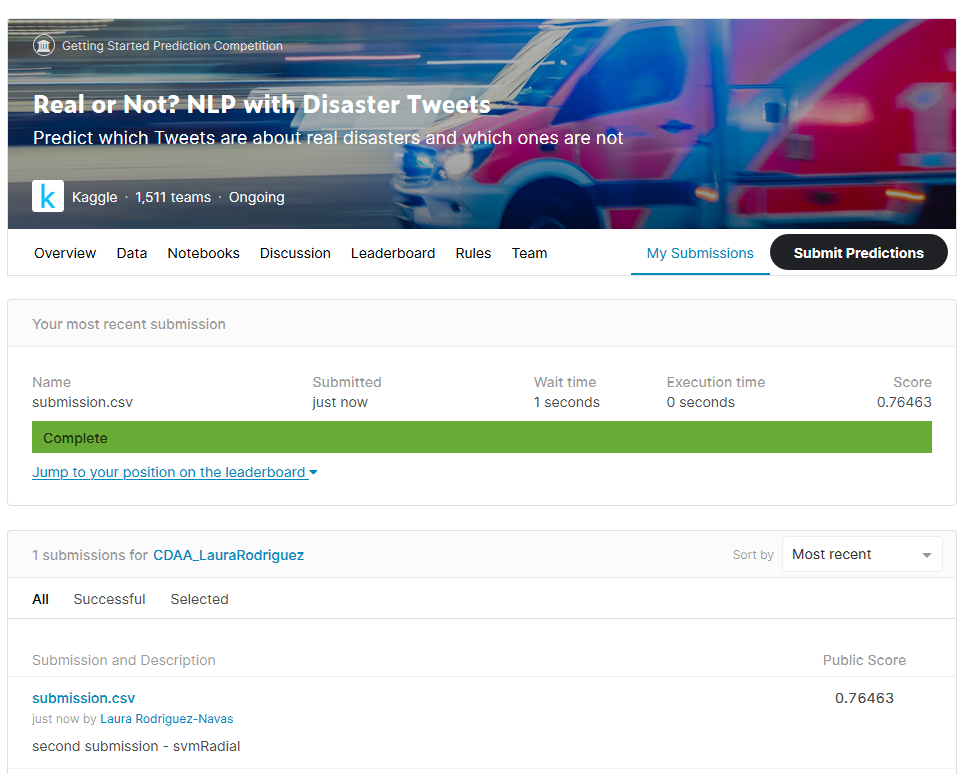
\includegraphics{submission.png}

\hypertarget{conclusiones}{%
\section{\texorpdfstring{\textbf{Conclusiones}}{Conclusiones}}\label{conclusiones}}

El resultado en Kaggle parece que es bueno. Realizar una técnica de
regresión lineal ha dado buenos resultados, aunque hay resultados mucho
mejores en Kaggle con la aplicación de otros modelos Un dato curioso es
que muchos de los usuarios de Kaggle utilizaron el modelo XGBoost. Me
pareció más entendedor utilizar un modelo binominal de regresión lineal
ya que se ha hablado de alguno durante la asignatura.

Además de los buenos resultados en Kaggle y del análisis del conjunto de
datos que me ayudó con la elección del modelo, la decisión de escoger el
modelo binominal de regresión lineal también se basó en el hecho de que
aún no había trabajado mucho usando una técnica de regresión lineal
durante la asignatura, así que me dio la posibilidad de aprender mucho
más. Sobretodo al hacer una evaluación del modelo, es muy difícil
evaluar. El trabajo se podría mejorar en este punto.

Otra de las cosas que consideré complicado y que me costó mucho fue la
selección de variables para la predicción. Había muchas opciones, al
final seleccioné la que me pareció más simple y que reducía mas el
conjunto de datos con una buena selección de variables. Ya que como
hemos visto en la asignatura la selección de variables es un proceso que
también es crucial para una buena predicción.

Que el trabajo se haya desarrollado en Kaggle le ha dado una motivación
extra.

\hypertarget{citas-para-fuentes-usadas}{%
\subsection{\texorpdfstring{\textbf{Citas para fuentes
usadas}}{Citas para fuentes usadas}}\label{citas-para-fuentes-usadas}}

\begin{itemize}
\tightlist
\item
  Notebook en Kaggle de xvivancos
  (\url{https://www.kaggle.com/xvivancos/kobe-bryant-shot-selection/}).
\item
  Notebook en Kaggle de khozzy
  (\url{https://www.kaggle.com/khozzy/kobe-shots-show-me-your-best-model/}).
\item
  Notebook en Kaggle de dixhom
  (\url{https://www.kaggle.com/dixhom/data-analysis-for-beginners/}).
\end{itemize}

\end{document}
